\section{Bioetica 1: Lezione introduttiva all'insegnamento di etica e deontologia}

\textbf{\emph{Le lezioni}}
\begin{itemize}
\item[1.] \textbf{ORDINE E PROFESSIONE}
\item[2.] \textbf{RISCHIO CLINICO E GESTIONE DEL RISCHIO CON ASPETTI ETICI}
\item[3.] \textbf{LA COMUNICAZIONE IN MEDICINA }
\item[4.] \textbf{IL CONTENZIOSO}
\end{itemize}

\subsection{Introduzione}

Il tema fondamentale di questo ambito è che spesso si sottovaluta un
aspetto importantissimo dell'essere medici, che è il saper essere. Il
sapere è declinato in diversi modi: sapere, saper fare e saper essere.
All'interno della bioetica vengono affrontati diversi temi, dallo studio
di tutto ciò che è vicino alla vita e che quindi entra nel sistema della
professione, all'emergente problema per cui ogni comportamento
dell'agire del medico deve essere etico.

{[}Il Professor Muzzetto commenta la percentuale di gradimento del
modulo di bioetica tra gli studenti, sottolineandone l'importanza. A tal
proposito cita l'organizzazione del corso di Medicina e Chirurgia del
mondo anglosassone, all'interno del quale il discorso di etica e
deontologia medica vine messo al primo posto.{]}

Un altro problema che verrà affrontato sarà il dilemma etico del curare
sempre o curare in base alla sostenibilità. Quello italiano è un sistema
universalistico, il cui significato è che ``chiunque abbia bisogno, qui
è accolto'', come recita il frontespizio dell'ospedale in Via Gramsci.
La nostra sanità tratta allo stesso modo il ricco e il povero. Anche
coloro che vengono da altre nazioni europee hanno diritto all'assistenza
sanitaria.

Altri due temi molto importanti sono il rapporto medico-paziente e
l'innovazione tecnologica (cioè come noi oggi ci dobbiamo porre di
fronte allo strumento informatico che va a sostituire in tutto e per
tutto i testi). Questo ha un significato rilevante: lo strumento ben
utilizzato è uno strumento prezioso, invece se è male utilizzato può
avere implicazioni negative e arrivare addirittura ad allontanarci dal
malato di persona. A tal proposito esiste l'e-visit, a causa del quale
non solo si fa la valutazione con un unico organo di senso, talvolta due
(vista e udito), ma si sta anche abbandonando ``l'utilizzo della mano''
e soprattutto la valutazione sulla persona mediante esame obiettivo. La
valutazione dell'uso dello strumento può portare a dilemmi etici.

Il rischio clinico è uno dei punti che crea problemi da un punto di
vista comportamentale. Molto spesso, come vedremo, il rischio clinico è
correlato alla mancanza di comunicazione tra colleghi.

La comunicazione spesso è carente e per questo ci si sta impegnando
molto a spiegare come deve essere la comunicazione ai giovani e futuri
medici.

Si parla di medicina \emph{difensiva} quandosi fa troppo perchè si ha
paura; di medicina \emph{desisitiva} perchè ci si astiene dal fare
determinate cose dando la responsabilità a terzi; di medicina
\emph{assicurativa} che è un argomento delicato in quanto con essa sono
sorti diversi problemi che hanno determinato un calo delle ``vocazioni''
(ci sono tutta una serie di specializzazioni che non vengono più scelte
dai neolaureati).

Oggi i medici sono chiamati a rispondere da un punto di vista etico al
concetto di salute. L'ottimizzazione delle risposte in termini di
qualità e durata della vita vanno a trasformare i desideri in bisogni e
a proporsi dei traguardi sempre più avanzati. L'evoluzione verso
l'invecchiamento, il decadimento e la morte portano alla consapevolezza
dell'esaurimento della vita; e questo porta al desiderio di salute.
Nella civiltà contemporanea la medicina che viene praticata travalica la
cura e si fa sempre più fatica a stabilirne i limiti. L'alta incidenza
della tecnologia ci porta a questa valutazione e purtroppo si sta
affermando nell'ambito della sostenibilità. L'economia diventa il
fattore limitativo dello sviluppo della medicina.

Infine tratteremo un argomento di cui non si parla mai, che è la
donazione del sangue. Infatti ci sono medici che non fanno fare la
trasfusione di sangue e non ne permettono la donazione. Questo è molto
grave. Quindi la donazione di sangue e la trasfusione sono sia un
fattore assistenziale che etico.

\subsection{Ordine e professione}

Il presidente dell'ordine dei medici è il presidente di un organo dello
stato ed il suo compito è quello di dare le basi ai giovani medici e a
coloro che esercitano. Il presidente dell'ordine insieme al relativo
consiglio si trova a giudicare il comportamento dei medici perchè non
sanno ``essere'' (ad es. il medico che straparla, che offende, che non
sa colloquiare). La maggior parte dei problemi originano perchè non
esiste un rapporto coerente tra medico e paziente. Alcuni potrebbero
chiedesii se il rapporto medico-pz esiste, persino nelle riviste di
settore tale rapporto viene messo in dubbio. Si sentirà parlare di
sostenibilità di sistema e di competenze assegnate ad altri ruoli:
significa che la società di oggi, impostata su base sociologica e mossa
dalla critica sociologica stessa (critica imperante nella sanità), porta
piano piano a staccare alcuni presupposti della professione medica per
darli ad altre figure professionali. Questo è un problema, e quindi
dobbiamo chiederci perchè alcune parti dell'attività medica vengono date
ad altre professioni. L'accademia e l'università, la professione e
l'ordine sono i due contrafforti su cui si fonda l'essere medico.
All'accademia bisogna imparare, ordine e professione rappresentano il
saper fare e il saper essere. Chi non si interessa a questi argomenti
(circa il 20\% di studenti ogni anno) non considera appieno il
significato di ``come saper fare il medico''. Il 95\% dei contenziosi
nascono perchè non si comunica. A fronte di questo problema bisogna
porre le basi affinchè non ci sia un avanzamento del problema, della
situazione di conflitto tra il medico e la società.

L'ordine è un ente autogestito e autofinanziato che ha il dovere di dire
a tutta la cittadinanza e a tutta la provincia quali sono i suoi compiti
e i problemi che deve risolvere quotidianamente. Svolge le seguenti
attività:

\begin{itemize}
\item
  \emph{Mantenimento dell'albo}: chi esercita la professione di Medico
  Chirurgo deve essere iscritto all'Ordine secondo la legislazione
  italiana, cioè è in possesso di tutti i titoli necessari. La funzione
  dell'albo quindi può essere riassunta in una funzione interna alla
  professione, cioè l'inquadramento del medico all'interno dell'Ordine,
  e in una funzione di natura pubblicistica, cioè il garantire
  l'idoneità allo svolgimento della professione. Svolge infine una
  funzione di garanzia verso i cittadini mettendoli a conoscenza delle
  persone che possono svolgere la professione. Un problema che si è
  presentato è che l'albo dei Medici e degli Odontoiatri sono entrambi
  sotto la responsabilità dell'Ordine dei Medici. É stata avanzata una
  proposta di legge affinché venga istituito anche un Ordine apposito
  per gli Odontoiatri.
\item
  \emph{Magistratura deontologica}: magistratura di tipo amministrativo
  che tutela il cittadino e tutela la professione. Interviene nelle
  segnalazioni fatte dal cittadino direttamente o tramite delega di un
  avvocato, oppure fatte tra colleghi medici. Garantisce che il medico
  abbia un comportamento consono ai criteri della professione sia per
  quanto concerne il suo essere medico che per quanto concerne il suo
  rapporto con la collettività.
\item
  \emph{Aggiornamenti nel post-laurea e formazione}: ogni anno bisogna
  acquisire 50 crediti per un totale di 150 crediti nel triennio
  frequentando convegni, allo scopo di rimanere
costantemente aggiornati. Chi non ottiene tali crediti viene sanzionato.
Ad esempio, a tutti i neolaureati e a tutti gli iscritti all'albo viene
fatto il corso di BLSD.
\end{itemize}

All'interno dell'Ordine vige il segreto d'ufficio.

L'Ordine, poiché è un organo dello Stato, ha la necessità di rapportarsi
con altre istituzioni come la Prefettura, il Comune, altre istituzioni
socio-sanitarie, la Magistratura, le Università e le Associazioni di
Volontariato, ad esempio per diffondere il proprio operato.

La Corte di Cassazione ha il compito di giudicare l'operato degli
ordini, approvando o cassando le loro decisioni o ancora consigliando di
rivalutarne alcuni aspetti.

Nello svolgere la professione si deve avere chiari quelli che
rappresentano i paletti del proprio agire. La professione deve
rispondere ad un codice deontologico, cioè un riferimento giuridico di
secondo livello. Dal giuramento di Ippocrate si passa all'etica
applicata rispettando le norme che la costituiscono. Il medico non può
prescindere da questo.

Nell'ambito deontologico, il problema è che ciascun medico crede di
avere i principi deontologici insiti in sé e si crea cosí un proprio
codice da seguire, convinto che sia l'unico corretto. Invece il codice
deontologico é unico per tutti ed é un autoregolamentazione della
professione. Per arrivare a definire tale codice si è preso in
considerazione il parere di tutte le parti sociali, dalle minoranze
religiose ai responsabili di tutte le associazioni, ai giuristi, ai
medici, ecc... il codice é nato da una condivisione di principi che sono
diventati la guida della professione medica. Quindi per legge è
diventato il sistema dei principi di etica medica che vanno a
disciplinare l'iter professionale del medico. È stata una scelta etica,
condivisa con la società. All'interno di questo codice ci sono
addirittura dei passi che vanno ad anticipare le leggi dello stato,
quindi significa che non è arretrato, ma all'avanguardia. Tali regole
devono essere rispettate. La prima regola è il rispetto stesso: il
rispetto dell'altro, della persona e dei colleghi. Quindi questo primo
principio costituisce la base della professione, ma ne rappresenta anche
uno dei punti deboli. Il codice ci dice le cose più importanti quali la
tutela della salute, il decoro e l'indipendenza della professione. Sono
dei termini che spesso sono sottovalutati. Il decoro nella professione
rappresenta l'esercizio della professione stessa secondo le regole, nel
rispetto altrui. Il medico quindi deve conoscere il codice ed è un
obbligo rispettarlo. Il primo atto di questo è il giuramento
professionale, che non è la lettura del giuramento di Ippocrate, ma è
l'impegno che ci si assume di fronte agli altri. È un atto di
responsabilizzazione, non di esibizionismo o di teatralità. Uno dei
problemi fondamentali del codice deontologico è stato l'enunciato del
"cosa deve o non deve fare il medico". Attorno a questo tema c'è un
fervore di pareri diversi. Non si può dire quello che il medico deve
fare. Però deve avere un comportamento fondato sulla tutela della salute
psicofisica, sul trattamento del dolore, sul sollievo delle sofferenze e
sul rispetto della libertà e della dignità della persona senza
discriminazione alcuna a prescindere dalle condizioni istituzionali e
sociali nelle quali lavora. Per poter fare tutto ciò servono delle
competenze esclusive legate alle pertinenze, alla formazione e alle
abilità. Quindi è necessario un percorso di formazione pre e
post-laurea. La diagnosi, la prevenzione e la terapia diventano parte
integrante delle competenze e sono indelegabili, anche in presenza di
strumenti tecnologici che possono indurre alla delega, alla commissione
e al controllo a distanza.

Ci sono alcuni articoli del codice che sono stati un po' modificati in
ambito di discussione perchè sono stati inseriti alcuni passaggi che si
possono prestare a interpretazione non coerente. Questo è uno dei
problemi per cui dovremo rivedere tali enunciati per renderli più chiari
(es. Art. 3).. In una situazione come questa il codice deontologico è
importantissimo.

Alla base del codice deontologico c'è il giuramento di Ippocrate.
Infatti se andate ad analizzarne i passi, vedrete che il codice
deontologico è costruito su di essi. Questo significa che 2500 anni di
storia della medicina hanno rafforzato, piuttosto che indebolito, il
concetto del medico e della sua funzione. La sintesi del codice la
troviamo nel nuovo giuramento professionale che parte dal rispetto e
dalla dignità delle persone e ripristina un concetto abbandonato: quello
di scienza e coscienza.

\begin{figure}[!ht]
\centering
	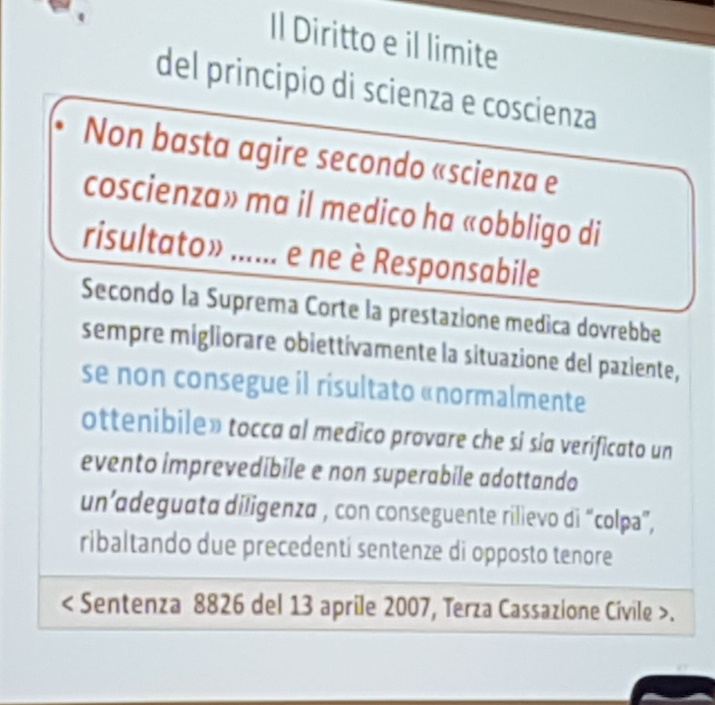
\includegraphics[width=0.8\textwidth]{29/image1.jpeg}
	\end{figure}

Agire in scienza significa essere aggiornati; agire in coscienza invece
significa dare un vero e proprio senso etico all'agire. La coscienza
diventa la sintesi deontologica dell'agire medico, richiamando un altro
concetto etico e professionale allo stesso tempo, ossia la
responsabilità del rapporto medico-paziente. Se un medico applica nel
suo modo di lavorare le linee guida dei protocolli è esonerato da
qualsiasi colpa in quanto tali linee guida sono state dimostrate essere
scientificamente le più efficaci.

Inoltre bisogna considerare che la cura di ogni patologia non dà una
risposta solo in base ad un aspetto terapeutico, ma anche in base alla
psicologia e alla personalità del paziente. Infatti vi troverete tante
volte davanti ad una situazione uguale a quella che si presentava spesso
in passato al momento dell'inserimento di un nuovo farmaco. Per esempio,
negli anni `78-'79, la cimetidina e la ranitidina rivoluzionarono da un
punto di vista terapeutico la patologia ulcerosa. Infatti fino a quel
momento, chi aveva l'ulcera veniva operato e subiva la gastroresezione.
Ora la diagnosi si fa in pochi minuti e con un farmaco il paziente può
tornare a lavorare in giornata. Questo è stato reso possibile dalla
cimetidina prima e dalla ranitidina poi. Ai pazienti fu prescritto in
principio il Ranitidil, successivamente venne anche prescritto lo
Zantac. Nonostante questi due farmaci siano in realtà lo stesso farmaco,
si assisteva ad un discreto numero di pazienti che riferiva di star male
e di non aver alcun giovamento dall'assunzione dello Zantac, mentre
traevano giovamento dall'assunzione del Ranitidil. Questo indica che da
un punto di vista psicologico, il paziente è molto più vulnerabile di
quello che si pensi.

\begin{figure}[!ht]
\centering
	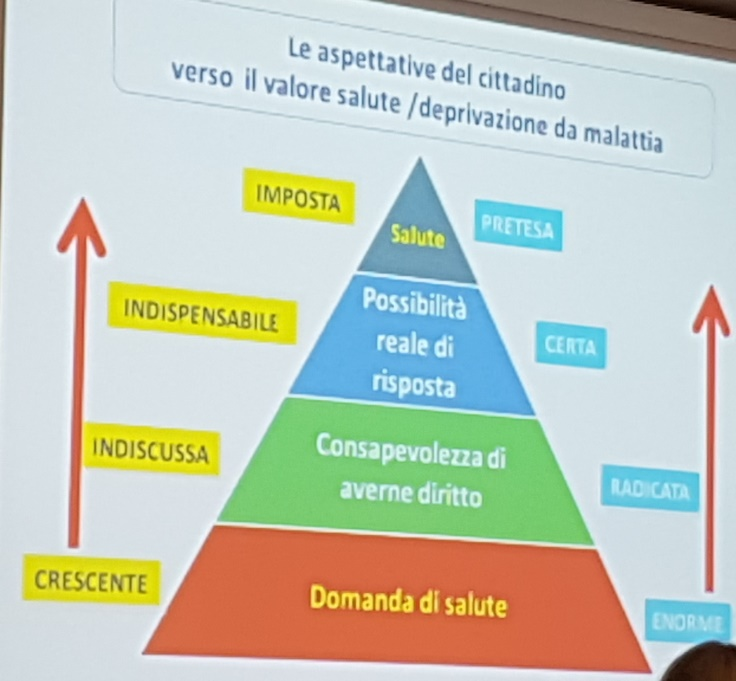
\includegraphics[width=0.8\textwidth]{29/image2.jpeg}
	\end{figure}

Oggi
i medici si trovano davanti ad aspettative sempre crescenti in termine
di salute. Il medico di oggi deve dipanare tale pretesa.

\begin{figure}[!ht]
\centering
	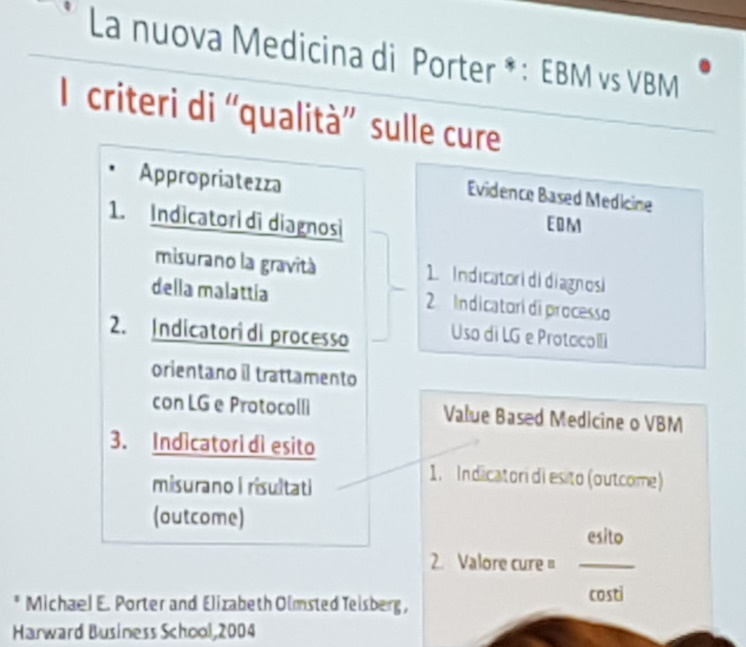
\includegraphics[width=0.8\textwidth]{29/image3.jpeg}
	\end{figure}

Ci
si sta spostando da una medicina basata sull'evidenza verso una medicina
basata sui risultati.

\begin{figure}[!ht]
\centering
	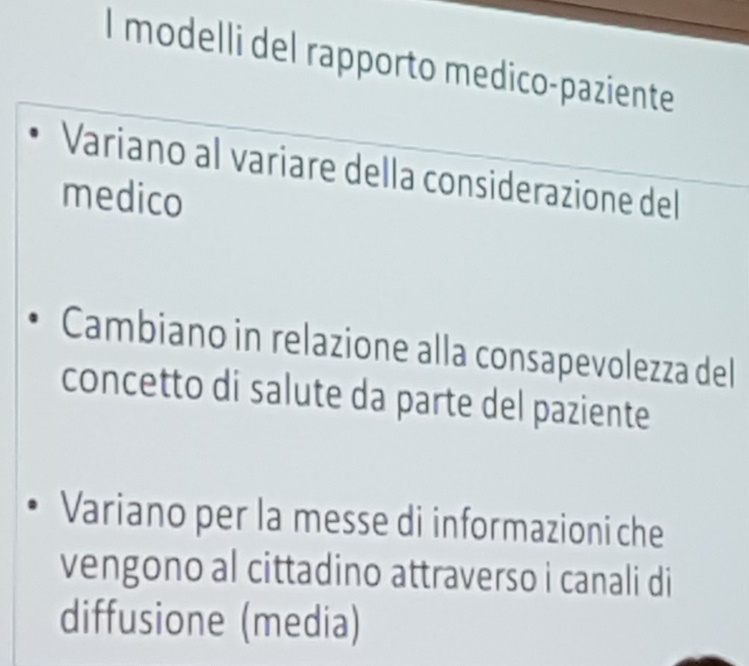
\includegraphics[width=0.8\textwidth]{29/image4.jpeg}
	\end{figure}

C'è inoltre un cambiamento nel rapporto medico-paziente legato alla
maggiore consapevolezza che ha il paziente del proprio stato di salute e
delle malattie, a tal punto da indurre i malati a presentarsi al medico
con un'autodiagnosi già formulata. Quindi sarà molto importante
smantellare il castello concettuale che ciascun malato si è fatto.

Un altro problema fortemente trascurato è quello dell'ascolto e della
comunicazione. Facendo un'indagine sui pazienti che venivano visitati ed
in particolare sull'ascolto attivo, si è evinto che per 80\% dei pz, il
tempo dedicato dal medico all'ascolto attivo è in media di due minuti.
Questo brevissimo lasso di tempo può orientare verso una diagnosi, ma
non è sufficiente per confermare quello che il paziente ha. Spesso
dall'ascolto del paziente si evincono numerosi elementi che non
emergerebbero da un ascolto superficiale, proprio perchè il pz è troppo
sovrastrutturato e quindi riferisce sintomi che appartengono
all'autodiagnosi che si è fatto e non che realmente accusa. È necessario
dedicare il giusto tempo all'ascolto del paziente per capire se nel
raccontare determinati sintomi finge o non finge. Il paziente finge in
buona fede e crede davvero di avere determinati sintomi. Togliere questa
sovrastruttura sintomatologica è molto difficile, ma si può fare ponendo
al paziente la stessa domanda riproposta più volte e in modi diversi.
Per fare ciò, la visita di 15 minuti diventa necessariamente una visita
di 30 minuti. Questo tempo non è mai speso male. Questo è tempo medico:
tempo dedicato all'ascolto, alla comunicazione e alla comprensione.
Questa è la base della caduta del rapporto medico-paziente da parte del
paziente. Molte persone fanno esposti all'Ordine che riguardano proprio
l'essere stati frettolosamente valutati dal medico. E questo è l'inizio
di un contenzioso. Secondo il codice questo è indelegabile ed è
responsabilità del medico. Se questo aspetto della professione verrà
sempre più delegato allora entrerà nel dimenticatoio la professione del
medico. Le nuove generazioni di medici devono assolutamente
salvaguardare questo aspetto per non trovarsi in difficoltà.

\begin{figure}[!ht]
\centering
	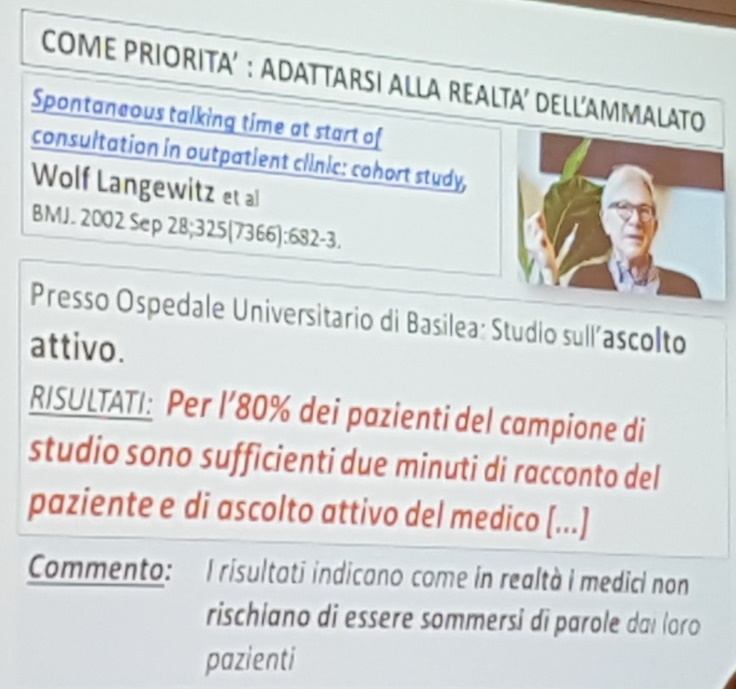
\includegraphics[width=0.8\textwidth]{29/image5.jpeg}
	\end{figure}
	
	\begin{figure}[!ht]
\centering
	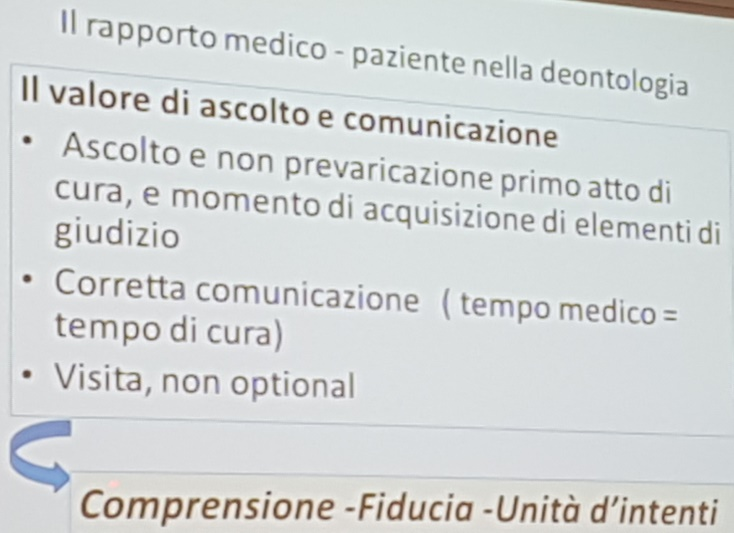
\includegraphics[width=0.8\textwidth]{29/image6.jpeg}
	\end{figure}

Il medico è una figura che può essere vista come un farmaco, di
conseguenza presenta un'azione farmacologica che ha anche degli effetti
collaterali. Poichè il rapporto medico-paziente nel tempo è stato messo
in crisi, la corte costituzionale è intervenuta difendendolo. I medici
hanno combattuto affinchè la corte costituzionale non trasformasse
questo rapporto In un rapporto medico-sanitario, dove l'atto medico
diventava un atto sanitario, cioè un atto disperso nelle decine di
professioni sanitarie esistenti. Tutto questo ci porta non soltanto alla
``negazionalitá'', all'equità, alla razionalità ed alla sperimentalità,
ma ci sprona ad essere responsabili. Un grande problema odierno è che i
medici non sono più capaci di ascoltare, di rispettare, e questo ci
viene ricordato da chi è deputato a dare un giudizio sulle professioni.
Questi giudizi vanno oltre il significato delle parole. Infatti se noi
medici veniamo richiamati circa determinati comportamenti, significa che
le persone atte a giudicare non vedono da parte nostra questi
comportamenti. Quindi se un comportamento non si vede di chi è la
responsabilità? É nostra e noi dobbiamo essere i primi ad agire per
correggere queste lacune, ovviamente senza esagerare. Infatti dobbiamo
sicuramente far sentire la nostra voce, ma dobbiamo rimanere dentro la
dimensione unificante della persona come entità. A tal riguardo uno dei
primi passaggi delle ultime stesure del codice deontologico è quello di
considerare il paziente una persona. Quindi non dobbiamo affrontare una
passaggio solamente di tipo sociologico o etico, ma si tratta della
considerazione, nella sua interezza, di chi sta male. Un tempo i
pazienti erano identificati con i numeri, successivamente con il nome
proprio, in seguito, per la privacy, si smise di utilizzare i nomi dei
pazienti sui letti e si tornò nuovamente al numero. Quindi siamo tornati
ad una situazione di ``spersonalizzazione'' della persona e questo è uno
dei problemi della medicina odierna.

Un'altra questione problematica è quella della pubblicitá. In passato
noi medici eravamo seri e severi circa la pubblicitá; al giorno d'oggi
invece, in seguito alla Legge Bersani, la concorrenza è alla base di
tutto. Tutto questo ha portato alla perdita del valore limite.
L'Authority ha dato alle federazioni degli Ordini 800 mila \euro{} di
multa perchè ponevano troppi divieti e paletti sulla pubblicità in
materia sanitaria contenuti nel codice deontologico del 2006 e nelle
Linee guida applicative, che secondo l'Antitrust costituiscono
\textless{}\textless{}illecite restrizioni della
concorrenza\textgreater{}\textgreater{}. Di conseguenza con una serie di
manovre abbiamo dovuto rimuovere il nostro decalogo della pubblicità e
siamo controllati dall'Authority perchè non osserviamo la concorrenza. É
indecente e indecoroso che un medico vada su un giornale a sostenere di
essere il migliore degli altri, un medico vale tanto quanto sa fare.
Molti medici che si pubblicizzano in questo modo sui giornali sono
convocati ancora oggi all'Ordine. Dobbiamo chiederci se ci sia bisogno
di tutto questo, oppure se dobbiamo entrare in una logica che ci spinga
a fare un esame di coscienza e a chiederci se siamo veramente a posto
con la nostra coscienza di medici. Ciò che io sto dicendo a voi oggi
sono le stesse parole che vengono rivolte a tutti i medici durante le
riunioni dell'Ordine in cui si affrontano questioni di etica. Si tratta
di dover applicare pochi principi, ma vi permetteranno di vivere
serenamente. Queste parole e questi principi di cui vi sto parlando oggi
saranno le basi della vostra professione e li dovrete conoscere ed
applicare.

\subsection{La comunicazione in medicina}

\begin{figure}[!ht]
\centering
	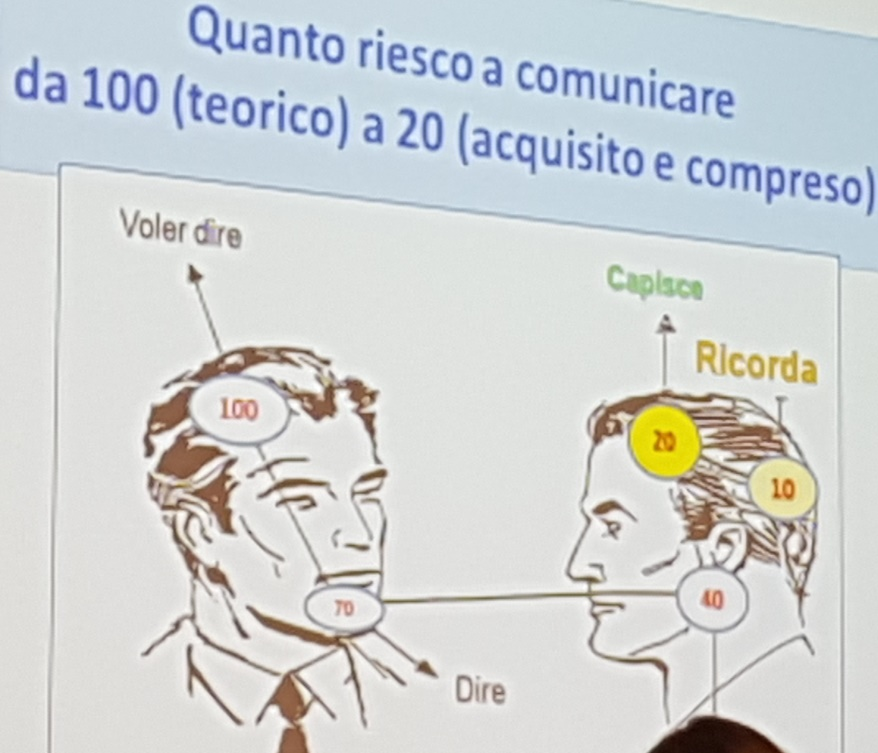
\includegraphics[width=0.8\textwidth]{29/image7.jpeg}
	\end{figure}

Circa la comunicazione tra due persone viene fatta una valutazione su
quante cose si vogliano dire e quante vengano dette. Ipotizziamo che ciò
che noi vogliamo dire sia quantificato con 100: noi siamo in grado di
esprimere probabilmente il 70\% del totale, per vari motivi: dal non
ricordare alcuni dettagli, al voler omettere delle parti. Di questo 70\%
i nostri interlocutori sono in grado di recepire circa il 40\%, e quanto
viene ricevuto dagli interlocutori deve essere compreso, e scendiamo
ulteriormente ad un 20\%, del quale viene memorizzato solamente il 10\%
del totale. Questo discorso serve ad illustrare e a giustificare il
fatto che ripetere cose, all'apparenza inutili, fa si che la percentuale
di quanto viene memorizzato aumenti. Ecco perchè ad ogni lezione vengono
presi degli appunti, cioé affinché rimanga di più. Alla luce di questo
saper ascoltare diventa un pregio, mentre saper ascoltare e saper capire
è una virtù. Quindi in quei pochi minuti di ascolto attivo è necessario
saper cogliere e fare una cernita di quanto e cosa viene detto.

Nel momento in cui noi ci troviamo a fare un'analisi di coscienza, il
rischio è che nel caso ci sia un errore, la responsabilità venga data a
qualcun altro. Infatti, come dicevamo prima, spesso ogni individuo si
crea un proprio codice deontologico, convincendosi di essere sempre nel
giusto. La conseguenza derivante da questo errore è il contenzioso (o
conflitto).

\subsection{Il rischio clinico}

\begin{figure}[!ht]
\centering
	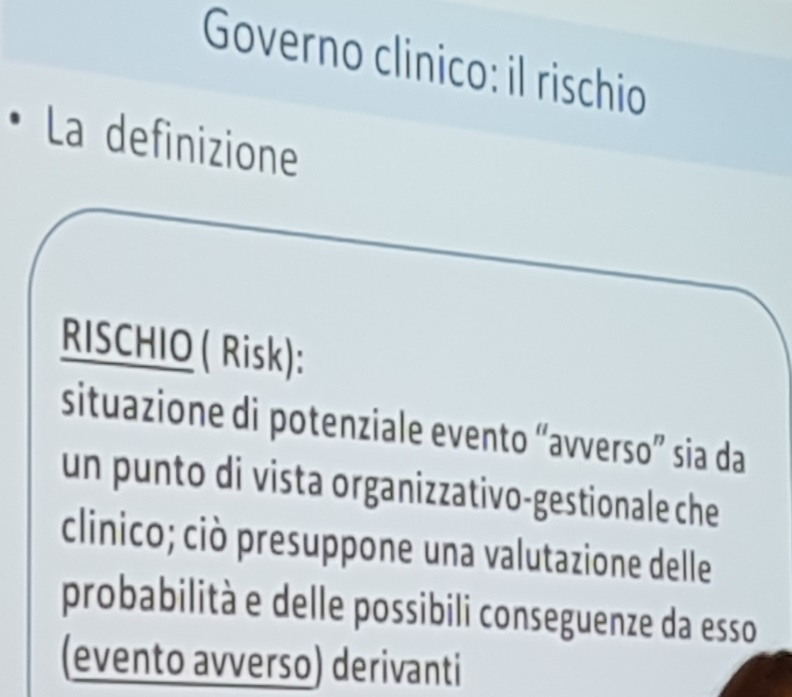
\includegraphics[width=0.8\textwidth]{29/image8.jpeg}
	\end{figure}

Il rischio clinico è una situazione in cui potenziali eventi gravi, se
non opportunamente controllati, si perpetuano e si manifestano. Ne
\emph{é} un esempio quello della Jolly Nero nel maggio del 2013. Si
tratta dell'incidente che capitò a Genova, quando una nave container
della linea Messina, durante le manovre, provocò la caduta della torre
di controllo del porto di Genova con numerosi morti. Questa nave
container, chiamata Jolly Nero, ebbe un problema durante le manovre,
mentre era trainata da un piccolo rimorchiatore. Purtroppo il
rimorchiatore non era abbastanza potente, quindi in prossimità alla
banchina non ebbe la capacità di contrastare l'abbrivio della nave, che
a sua volta colpí la banchina. Questo accadde il 7 maggio 2013 e la
causa fu il blocco dei motori della nave container. Un mese dopo la
Jolly Nero, tornata al terminal Messina, ebbe nuovamente un un blocco
dei motori. Tuttavia in questa occasione, dopo l'episodio dell'incidente
del mese precedente, la nave container non era trainata da un piccolo
rimorchiatore, ma da uno di maggior portata. In questo modo la nave
ruscì a frenare, impedendo un'altra tragedia. Da questo fatto di cronaca
possiamo dedurre che grazie alla conoscenza di un fatto sfavorevole e
grave si può evitare che si ripresenti. Purtroppo pare che in precedenza
ci fossero stati dei casi analoghi mai stati segnalati di
malfunzionamento ai motori. Queste segnalazioni mancate hanno avuto come
conseguenza la tragedia nel porto di Genova. Questo esempio illustra
cos'è il rischio clinico. Un evento possibile che per un qualsiasi
motivo non si avvera (un incidente evitato), se utilizzato per informare
chi di dovere, può permettere di evitare che quell'evento si verifichi
in futuro. Non è necessario che ci sia una tragedia affinchè si possa
capire che si tratta di un evento presagio di una situazione drammatica.
Il vero problema che dobbiamo affrontare è che quel fenomeno non si
verifichi. Questo è il principio che sta alla base di tutto il percorso
formativo che c'è nel percorso di gestione del rischio clinico. Il
Sistema Sanitario è complesso perchè comprende molte persone, perchè si
utilizzano molti strumenti, perchè c'è correlazione ed interazione tra
tutte le persone e le strumentazioni comprese nel sistema sanitario.
Quindi se non è presente una logica che renda omogeneo il rapporto e lo
metta in sicurezza, se manca quindi una valutazione del rischio che
impedisca al rischio di verificarsi, allora il sistema sanitario fa
acqua.
